\documentclass[]{article}
\usepackage[top=1in, bottom=1.25in, left=1.25in, right=1.25in]{geometry}
\usepackage{hyperref}
\usepackage{amsfonts}
\usepackage{amsmath}
\usepackage{graphicx}
\usepackage{float}
\usepackage{bbm}

\usepackage{listings}
\usepackage{color}

\definecolor{dkgreen}{rgb}{0,0.6,0}
\definecolor{gray}{rgb}{0.5,0.5,0.5}
\definecolor{mauve}{rgb}{0.58,0,0.82}

\lstset{frame=tb,
	language=Python,
	aboveskip=3mm,
	belowskip=3mm,
	showstringspaces=false,
	columns=flexible,
	basicstyle={\small\ttfamily},
	numbers=none,
	numberstyle=\tiny\color{gray},
	keywordstyle=\color{blue},
	commentstyle=\color{dkgreen},
	stringstyle=\color{mauve},
	breaklines=true,
	breakatwhitespace=true,
	tabsize=3
}

\title{\textbf{Decision trees}}
\author{Yacine Debbabi}

\begin{document}

\maketitle

\tableofcontents


\section{Tree models}

Consider our data consists of $p$ inputs and a response for $N$ observations. We model the response as a constant-by-part function in $M$ distinct regions, i.e.
\begin{eqnarray}
f(x)=\sum_{m=1}^M c_m \mathbbm{1}(x\in R_m).
\end{eqnarray}
Here we first show how to estimate the response for a given set of regions, and then discuss how trees can be used to build region splits.

\section{How to estimate a tree response?}

We estimate $\hat{c}=(\hat{c}_1,...,\hat{c}_M)$ in each region by minimizing an impurity/loss function, i.e.
\begin{equation}
\hat{c}_m = \mathrm{argmin}_c Q_m(c)
\end{equation}
for each $m\in{1,...,M}$. For regression problems, this is is often chosen as a residual sum of squares, i.e.
\begin{equation}
Q_m(c) = \frac{1}{N_m}\sum_{x_i\in R_m} (y_i-c)^2.
\end{equation}
The solution $\hat{c}_m$ is easily obtained, by differentiating $Q_m(c)$ against $c$, as the average of responses $y_i$ whose input $x_i$ lie in $R_m$. For classification problems, we classify the observations in node $m$ to class $\hat{k}_m=\textrm{argmax}_k \hat{p}_{k,m}$, where $\hat{p}_{k,m}$ denotes the proportion of class $k$ observations in node $m$. Impurity is often quantified using the misclassification rate
\begin{equation}
Q_m(c) = \frac{1}{N_m}\sum_{x_i\in R_m} \mathbbm{1}(y_i \neq c),
\end{equation}
when cost-complexity pruning the tree (see later but not sure why), and using the Gini index
\begin{equation}
Q_m(c) = \sum_{k\neq k'} \hat{p}_{k,m}\hat{p}_{k',m}
\end{equation}
when growing the tree. The Gini index is preferable for such task because (a) it is differentiable (and hence more amenable to numerical optimization), and (b) more sensitive to node probabilities than the misclassification rate. The latter can be further demonstrated by comparing two scenarios: (a) (100,300) vs (100,300) splits, and (b) (200,400) vs (200,0) splits. Both scenarios show the same misclassification rate but a lower Gini index for the second scenario.

\section{How to grow a tree?}

\noindent We now discuss how to grow a regression tree. Finding a multi-region partition that minimizes impurity is generally computationally infeasible. Hence we proceed with a greedy algorithm. Starting with all the data, we consider a splitting variable $j$ and a split point $s$, and define the half planes $R_1(j,s)=\{ X | X_j\leq s\}$ and $R_2(j,s)=\{ X | X_j>s\}$. Then we seek the splitting variable and point that solve
\begin{eqnarray}
\min_{j,s}\left[\min_{c_1} N_{m_1}Q_{m_1}(c_1)+\min_{c_2} N_{m_2}Q_{m_2}(c_2) \right].
\end{eqnarray}
For each splitting variable $j$, the $j$-feature observations $x_i^j$, $i=1,...,N$, can be sorted, and the objective function be evaluated on splitting points $s$ sampled from the $j$-feature values. The procedure can be repeated separately on the subregions, and the resulting region splits can be represented as a binary tree.

\begin{lstlisting}
from sklearn.datasets import load_boston
from sklearn.tree import DecisionTreeRegressor, plot_tree

X, y = load_boston(return_X_y=True)

regressor = DecisionTreeRegressor(
    criterion="mse",
    max_depth=2, 
    min_samples_leaf=10,
).fit(X, y)

plot_tree(regressor)
plt.show()
\end{lstlisting}

\begin{figure}[H]
\center 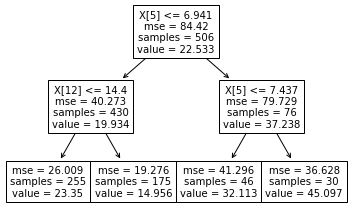
\includegraphics[scale=1]{tree-example}
\caption{Example of regression decision tree.}
\end{figure}

\noindent When shall we stop growing a tree? Clearly a very large tree might overfit the data, while a small tree might not capture the important structure. The preferred strategy is to grow a large tree $T_0$, which is then pruned. Although fully grown and unpruned trees can potentially be very large on some data sets, we usually cap the depth of the tree and/or the minimum number of observations in each region. This helps reduce memory consumption and training runtimes.

\section{How to prune a single tree?}

\noindent We now discuss the \textbf{cost-complexity pruning} approach. We define a subtree $T\subset T_0$ to be any tree that can be obtained by pruning $T_0$, i.e. by removing any number of its internal (non-terminal) nodes (and their descendants). A pruned tree is obtained by minimizing the cost-complexity criterion
\begin{equation}
\hat{T}_\alpha = \textrm{argmin}_T \hspace{1pt} \sum_{m=1}^{|T|} N_m Q_m(T) + \alpha |T|,
\end{equation}
where $m$ indexes the terminal nodes and $|T|$ denotes the number of terminal nodes of tree $T$. This is achieved with the \textbf{weakest link pruning} approach; this is discussed further \href{https://online.stat.psu.edu/stat508/lesson/11/11.8/11.8.2}{here}. One can show the solution is unique. Estimation of $\alpha$ is achieved by cross-validation.

\section{How to quantify the relative importance of features?}

For a single decision tree $T$, the relevance of predictor variable $X_l$ is defined as
\begin{equation}
I_l^2(T):= \sum_m i^2_m \mathbbm{1}(\textrm{f splits m})
\end{equation}
where $m$ is an internal node of $T$ and $i^2_m$ is the increase in $N_mQ_m$ which is obtained from the split. This is generalized for a forest by averaging the above over all trees.

\section{Random forests}

Random forests are built by constructing a set of trees randomly, by randomly selecting a fixed-size set of feature candidates, and "averaging" their predictions. 

\begin{figure}[H]
	\center 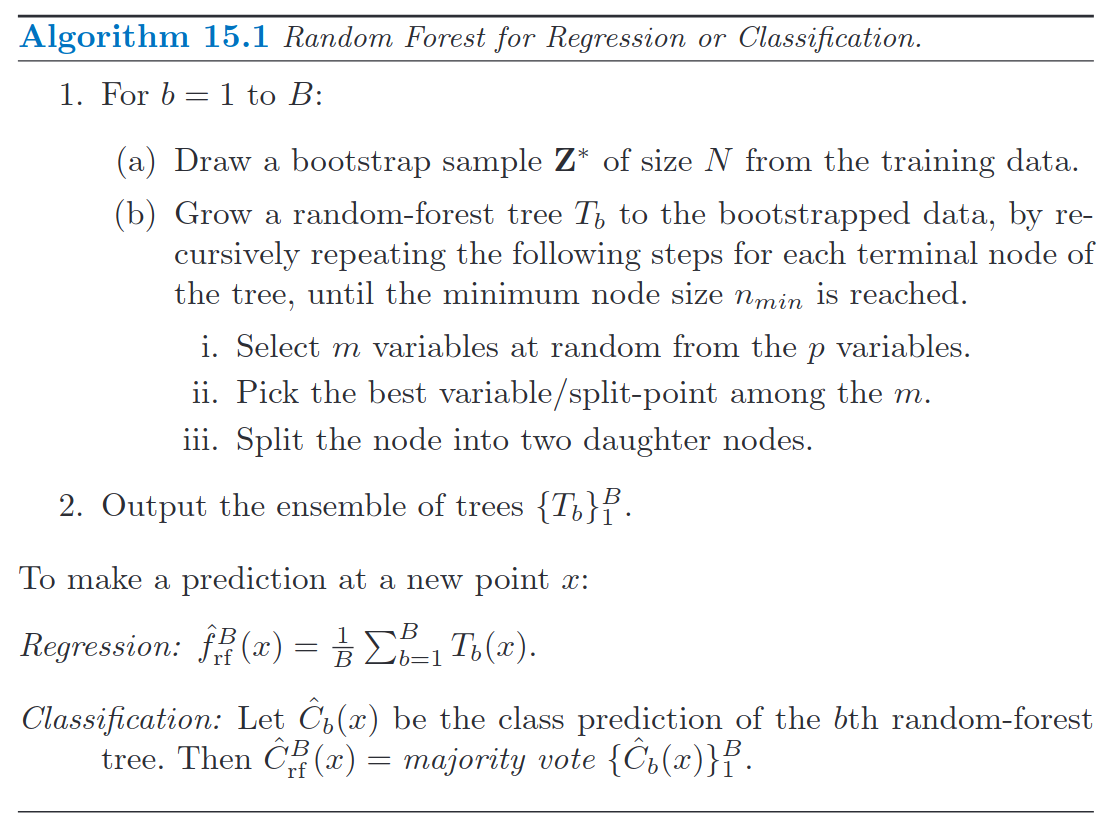
\includegraphics[scale=.25]{random-forests}
	\caption{Random forest construction algorithm.}
\end{figure}

\noindent The parameters to tune are (a) the number of trees, (b) the max number of feature candidates, and (c) (single) tree depth parameters. Random forests allow estimation of an "out-of-bag" (OOB) error. An error is calculated for each sample by averaging the trees which did not use this sample for training. We empirically find in general that the OOB error converges as we increase the number of trees. This can be used to derive an upper bound of the number of trees required. The other parameters can be optimized by cross-validation using the GridSearchCV estimator.

\begin{lstlisting}
from sklearn.ensemble import RandomForestRegressor

params = {
	"n_estimators": 100,
	"max_features": "sqrt", 
	"max_depth": 4, 
	"oob_score": True, 
	"random_state": 0, 
	"max_samples": .8    
}

# 

oob_scores = []
n_est_grid = [int(x) for x in np.logspace(1.2, 3, 20)]

for n in n_est_grid:
	params.update({"n_estimators": n})
	rf = RandomForestRegressor(**params).fit(X, y)
	oob_scores.append(rf.oob_score_)

plt.semilogx(n_est_grid, oob_scores, "bo-")
plt.xlabel("Number of trees"); plt.ylabel("OOB score"); plt.show()

# Hyperparameter optimization

from sklearn.model_selection import GridSearchCV

gs = GridSearchCV(estimator=rf, param_grid={"n_estimators": [100], "max_depth": [2, 4, 6], "max_features": ["auto", "sqrt"]}, cv=5).fit(X, y)
gs.best_estimator_
\end{lstlisting}

\begin{figure}[H]
	\center 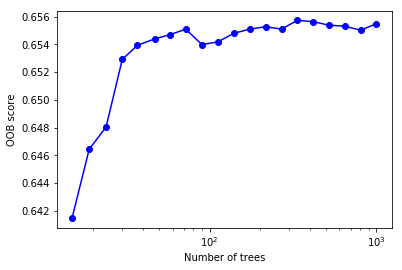
\includegraphics[scale=.7]{RF_OOB_scores_CV}
	\caption{OOB scores converge as we increase the number of trees.}
\end{figure}

\end{document}
